\lhead{\begin{tikzpicture}[remember picture, overlay]
    \node [anchor=100,inner sep=0] (imagenIZQUIERDA) at (current page header area.north){
\includegraphics[width=18cm]{img/Encabezado.PNG}};
    \end{tikzpicture}}
    \rhead{Ángeles-Hurtado}
    \rfoot{\begin{tikzpicture}[remember picture, overlay]
    \node [anchor=140,inner sep=0] (imagenDERECHA) at (current page footer area.south){
\includegraphics[width=18cm]{img/Foot.PNG}};
    \end{tikzpicture}}
    %----------------------------------------------------------------------------------------
    \lfoot{ \thepage}
    % \renewcommand{\labelenumi}{\alph{enumi}.)} 
    %----------------------------------------------------------------------------------------
    %----------------------------------------------------------------------------------------
    %	TITLE SECTION
    %----------------------------------------------------------------------------------------
    
    \setlength{\droptitle}{-5\baselineskip} % Move the title up
    \title{\textbf{Estudio de tiempos y movimientos en el ensamble de un circuito electrónico utilizando diferentes métodos para su optimización }} % Article title
    
     \author{ 
     \textsc{Sáenz-Saavedra, Kenia Paola}\\ 
    %  Afiliación:
     \texttt{ Instituto Tecnológico de Querétaro } \\ 
     \texttt{Tecnológico Nacional de México} \\ 
     \texttt{Querétaro, México}\\ 
     \texttt{l22140911@queretaro.tecnm.mx} 
     \and 
     \textsc{Ángeles-Hurtado, Luis Alberto}\\ 
    %  Afiliación:
     \texttt{ Instituto Tecnológico de Querétaro } \\ 
     \texttt{ Tecnológico Nacional de México } \\ 
     \texttt{Querétaro, México}\\ 
     \texttt{alb3rt0.ah@gmail.com} 
    }
    
    
    %----------------------------------------------------------------------------------------
    
    % \begin{document}
    
    % Print the title
    \maketitle
    \thispagestyle{fancy}
    
    %----------------------------------------------------------------------------------------
    %	ARTICLE CONTENTS
    %----------------------------------------------------------------------------------------
    
    % \section*{Resumen}
    % \textit{Palabras clave:}
    % El resumen (ancho de página) deberá contener entre 100 y 200 palabras tipo Adobe Devangari 11 puntos.
    
    \begin{abstract}
    \noindent 
    El resumen (ancho de página) deberá contener entre 100 y 200 palabras tipo Adobe Devangari 11 puntos.
    
    \end{abstract}
    % 
    % 
    \textbf{\textit{Palabras clave}}: {First keyword should be the corresponding to the research area according with the authors guide. Maximum of 6 keywords.}
    % \keywords{First keyword should be the corresponding to the research area according with the authors guide. Maximum of 6 keywords.}
    \begin{itemize}
        \item Estándar, preciso, exacto, optimización, proceso.
    \end{itemize}
    
    \section{Introducción}
    \begin{itemize}
        \item Estudio de Tiempos Y Moviminetos: El estudio de tiempo y movimiento es una herramienta la cual sirve para determinar los tiempos estándar de cada una de las operaciones que componen cualquier proceso, así como para analizar los movimientos que son realizados por parte de un operario para llevar a cabo dicha operación.
        \item  Ensamble: Un proceso de ensamble implica la colocación de dos o más piezas individuales para la conformación de un producto final. Suele dividirse en niveles dependiendo de la cantidad de componentes a unir, ya sean mecánicos, de software, electrónicos, farmacéuticos, o de cualquier otro tipo
        \item Circuito Electrónico: Un circuito eléctrico o red eléctrica, es una colección de elementos eléctricos interconectados de alguna forma específica. 
        \item Método de tiempos predeterminados: Consisten en una base de datos de tiempos de movimientos básicos.Se asignan tiempos estándar a los elementos básicos del trabajo. Se asignan a los movimientos fundamentales y a grupos de movimientos que no se pueden evaluar con precisión mediante los procedimientos ordinarios de estudio de tiempos con cronómetro. También son el resultado de estudiar una muestra grande de operaciones diversificadas con un dispositivo de ritmo como una cámara de filmación o videograbación, capaz de medir elementos muy cortos.
        \item Buscar la mejor manera de realizar una actividad, lo más eficientemente posible, con la menor cantidad de recursos.
    \end{itemize}
     
    % Define estudio de tiempos y movimientos
    % define que es ensamble
    % define que es circuito electronico
    % define el metodo de tiempos predeterminados
    % define optimización
    \begin{itemize}
    
    
         \item Una de las técnicas más utilizadas para superar deficiencias y elevar la productividad de los trabajadores es el estudio del trabajo, definido como el examen sistemático de los métodos para realizar actividades con el fin de mejorar la utilización eficaz de los recursos y de establecer normas de rendimiento con respecto a las actividades que se están realizando, tuvo sus orígenes a principios del siglo XX, con los trabajos realizados por Frederick W. Taylor y continuados unos años después por los esposos Gilbreth (Kanawaty, 1996). Esta actividad implica la técnica de establecer un estándar de tiempo permisible para realizar una tarea determinada, con base en la medición del contenido de trabajo del método prescrito, con la debida consideración de la fatiga y las demoras personales y los retrasos inevitables (Niebel \& Freivalds, 2014).
        \item La metodología que se llevó a cabo en en este estudio de tiempos y movimientos fué: Principalmente el ensamble que se analizaría, posteriormente estudiar los componentes a este. Aplicando un estudio de tiempos y movimientos mediante la técnica de cronómetro a vuelta cero y describiendo las actividades que permitan un procedimiento sistemático. en base esto se analizan los resultados obtenidos y se hacen las modificaciones pertinentes eliminando los movimientos ineficientes logrando una mayor productividad. 
        
        \item El estudio de tiempos con cronómetro de forma tradicional, representa la técnica más utilizada como elemento de medición de las tareas, encontrándose más del 89\% de los trabajos desarrollados bajo ésta técnica.
        La aplicación del estudio de tiempos y movimientos sigue teniendo vigencia en la actualidad, como lo demuestran las 66 investigaciones realizadas entre los años 2010–2016, las cuales aplicaron las técnicas de medicióndel trabajo en sus formas tradicionales de muestreo del trabajo, estudio de tiempos con cronómetro y estándares de tiempo predeterminados.
        \item El estudio que se realiza en este proyecto integrador tuvo cómo objetivo principal llevar a la práctica los conociminetos adquiridos a lo largo de estos 4 semestres, involucrando las materias y talleres ya cursados en la carrera. De igual manera a través de este ensamble desarollar nuevas habilidades adquiridas en la materia de Estiudio del Trabajo II. Aplicando lo anterior mencionado, obtener buenos resultados atraves del del estudio, logrando una optimización en este proceso.
        \item Debe de tener Referencias científicas, URL, tesis, etc.
    \end{itemize}
    % 
    % 
    \section{Justificación}
    
    \begin{itemize}
        \item El entorno global ha llevado a las organizaciones a buscar la mejora de sus procesos por medio de la identificación y eliminación en forma gradual de las actividades que no generan valor a sus productos y procesos. Estas actividades representan costos operacionales que se traducen en despilfarros de tiempo, materiales, espacio y demás recursos organizacionales. Una de las técnicas más utilizadas para superar dichas deficiencias y elevar la productividad de los trabajadores es el estudio del trabajo.
        
        Se debe de describir lo que se requiere, lo que se necesita o lo que se demanda en la actualidad con un enfoque global pero terminar con menciones a temas locales o nacionales.
        \item Debe de tener Referencias científicas, URL, tesis, etc.
    \end{itemize}
    % 
    % 
    \section{Descripción del problema}
    \begin{itemize}
        \item Se debe describir la desviación o diferencia del ``es'' con respecto al ``debe ser''.
        \item Se debe hacer alusión a la incógnita científica*.
        \item Debe de tener Referencias científicas, URL, tesis, etc.
    \end{itemize}
    
    \textbf{*La incógnita científica es el elemento cuya solución incrementa el conocimiento científico.}
    % 
    % 
    \section{Fundamentación teórica}
    
    Es la parte medular y de mayor discusión, deberá ser la fundamentación de la hipótesis, por tanto se deberá señalar claramente la razón de la suposición y fundamentación de la misma. Únicamente referencias científicas.
    \begin{itemize}
        \item Se debe de retomar el tema que se planteo en la introducción, pero ahora profundizando para clarificar la incógnita científica y se pueda plantear la hipótesis.
        \item Se debe de retomar la descripción del problema, pero ahora a profundidad del (los) objeto(s) de estudio. 
        \item Se debe de profundizar en las metodologías que se ha usado para el estudio del tema.
        \item Referencias solo de artículos y libros científicos.
    \end{itemize}
    % 
    % 
    \section{Hipótesis}
    
    Es la suposición con fundamento científico relativa a la solución del problema, necesidad o de cómo se aprovecha la oportunidad con la incógnita científica y se fundamenta con: 1. Una suposición (en afirmativo o negativo) y ésta deberá vincularse con:
    2. La fundamentación científica que deberá ser precisa 3. Una entidad de comparación para probar la suposición y
    4. La variable con que se califica o cuantifica la comparación o se prueba la hipótesis.
    
    \begin{itemize}
        \item Se debe de identificar claramente la suposición científica
        \item Se debe de identificar claramente el fundamento científico
        \item Se debe identificar claramente la variable de respuesta
        \item Se debe identifican claramente las realidades o modelos contrastantes
        \item Se debe de establecer las variables asociadas, explicativas o que tienen relación funcional con la variable de respuesta
    \end{itemize}
    % 
    % 
    \section{Objetivo}
    
    Realizar un estudio de tiempos y movimientos de un ensamble eléctrico para a partir de este análisis eliminar los movimientos ineficientes, eliminar tiempos muertos y aumentar la productividad, de esta manera comprobando la hipótesis planteada.
    \begin{itemize}
        \item Se debe establecer que se pretende probar la hipótesis
    \end{itemize}
    
    \subsection{Objetivos específicos }
    
    \begin{itemize}
        \item Aplicar los conocimientos adquiridos en otras materias cursadas.
        \item Implementar nuevas herramientas y software para la elaboración del proyecto integrador.
        \item  Adquirir mayor capacidad de análisis y síntesis.
        \item Desarrollar habilidades de autonomía y adaptación al cambio así como a métodos nuevos.
    \end{itemize}
    
    Son actividades orientadas al cumplimiento del objetivo general. Se establecen con verbos activos en infinitivo. Son parte de la acción encaminada a probar la hipótesis. Éstos deben ser precisos, y en lo posible evitar aspectos metodológicos.
    % 
    % 
    \section{Cuerpo (Metodología, modelo matemático, etc.)}
    
    Cada estrategia metodológica se establece acorde a cada objetivo, y por tanto deberá ser desglosada precisada y ordenada claramente. En consecuencia cada objetivo que se presentó en forma de verbo en infinitivo deberá determinar una estrategia en forma de adverbio. Ej. Desarrollar…Desarrollo. Son las actividades ordenadas que tienen como finalidad la prueba de la hipótesis. 
    
    \begin{itemize}
        \item Se debe establecer que se habrá de hacer, como, conque, y donde para obtener la información que permita probar la hipótesis.  
        \item Se debe desglosar de acuerdo a los objetivos específicos. 
        \item Se debe establecer una estrategia metodológica por cada objetivo específico. De manera simplista se podría decir que se cambia el verbo en infinitivo por su respectivo adverbio.
        \item En cada objetivo se debe describir que método, que materiales y que equipo se usará para conseguirlo.
        \item Se deben tener referencias Figura \ref{fig:lcd-16x2}.
    \end{itemize}
    % 
    % 
    \begin{figure}[H]
        \centering
        \includegraphics[trim = {3mm 6mm 9mm 2mm},clip,scale=0.5]{32/Img/ESP 32 PDF.PDF}
        \caption{Esquema LCD de 16x2}
        \label{fig:lcd-16x2}
    \end{figure}
    % 
    % 
    % \begin{figure}[H]
    %     \centering
    %     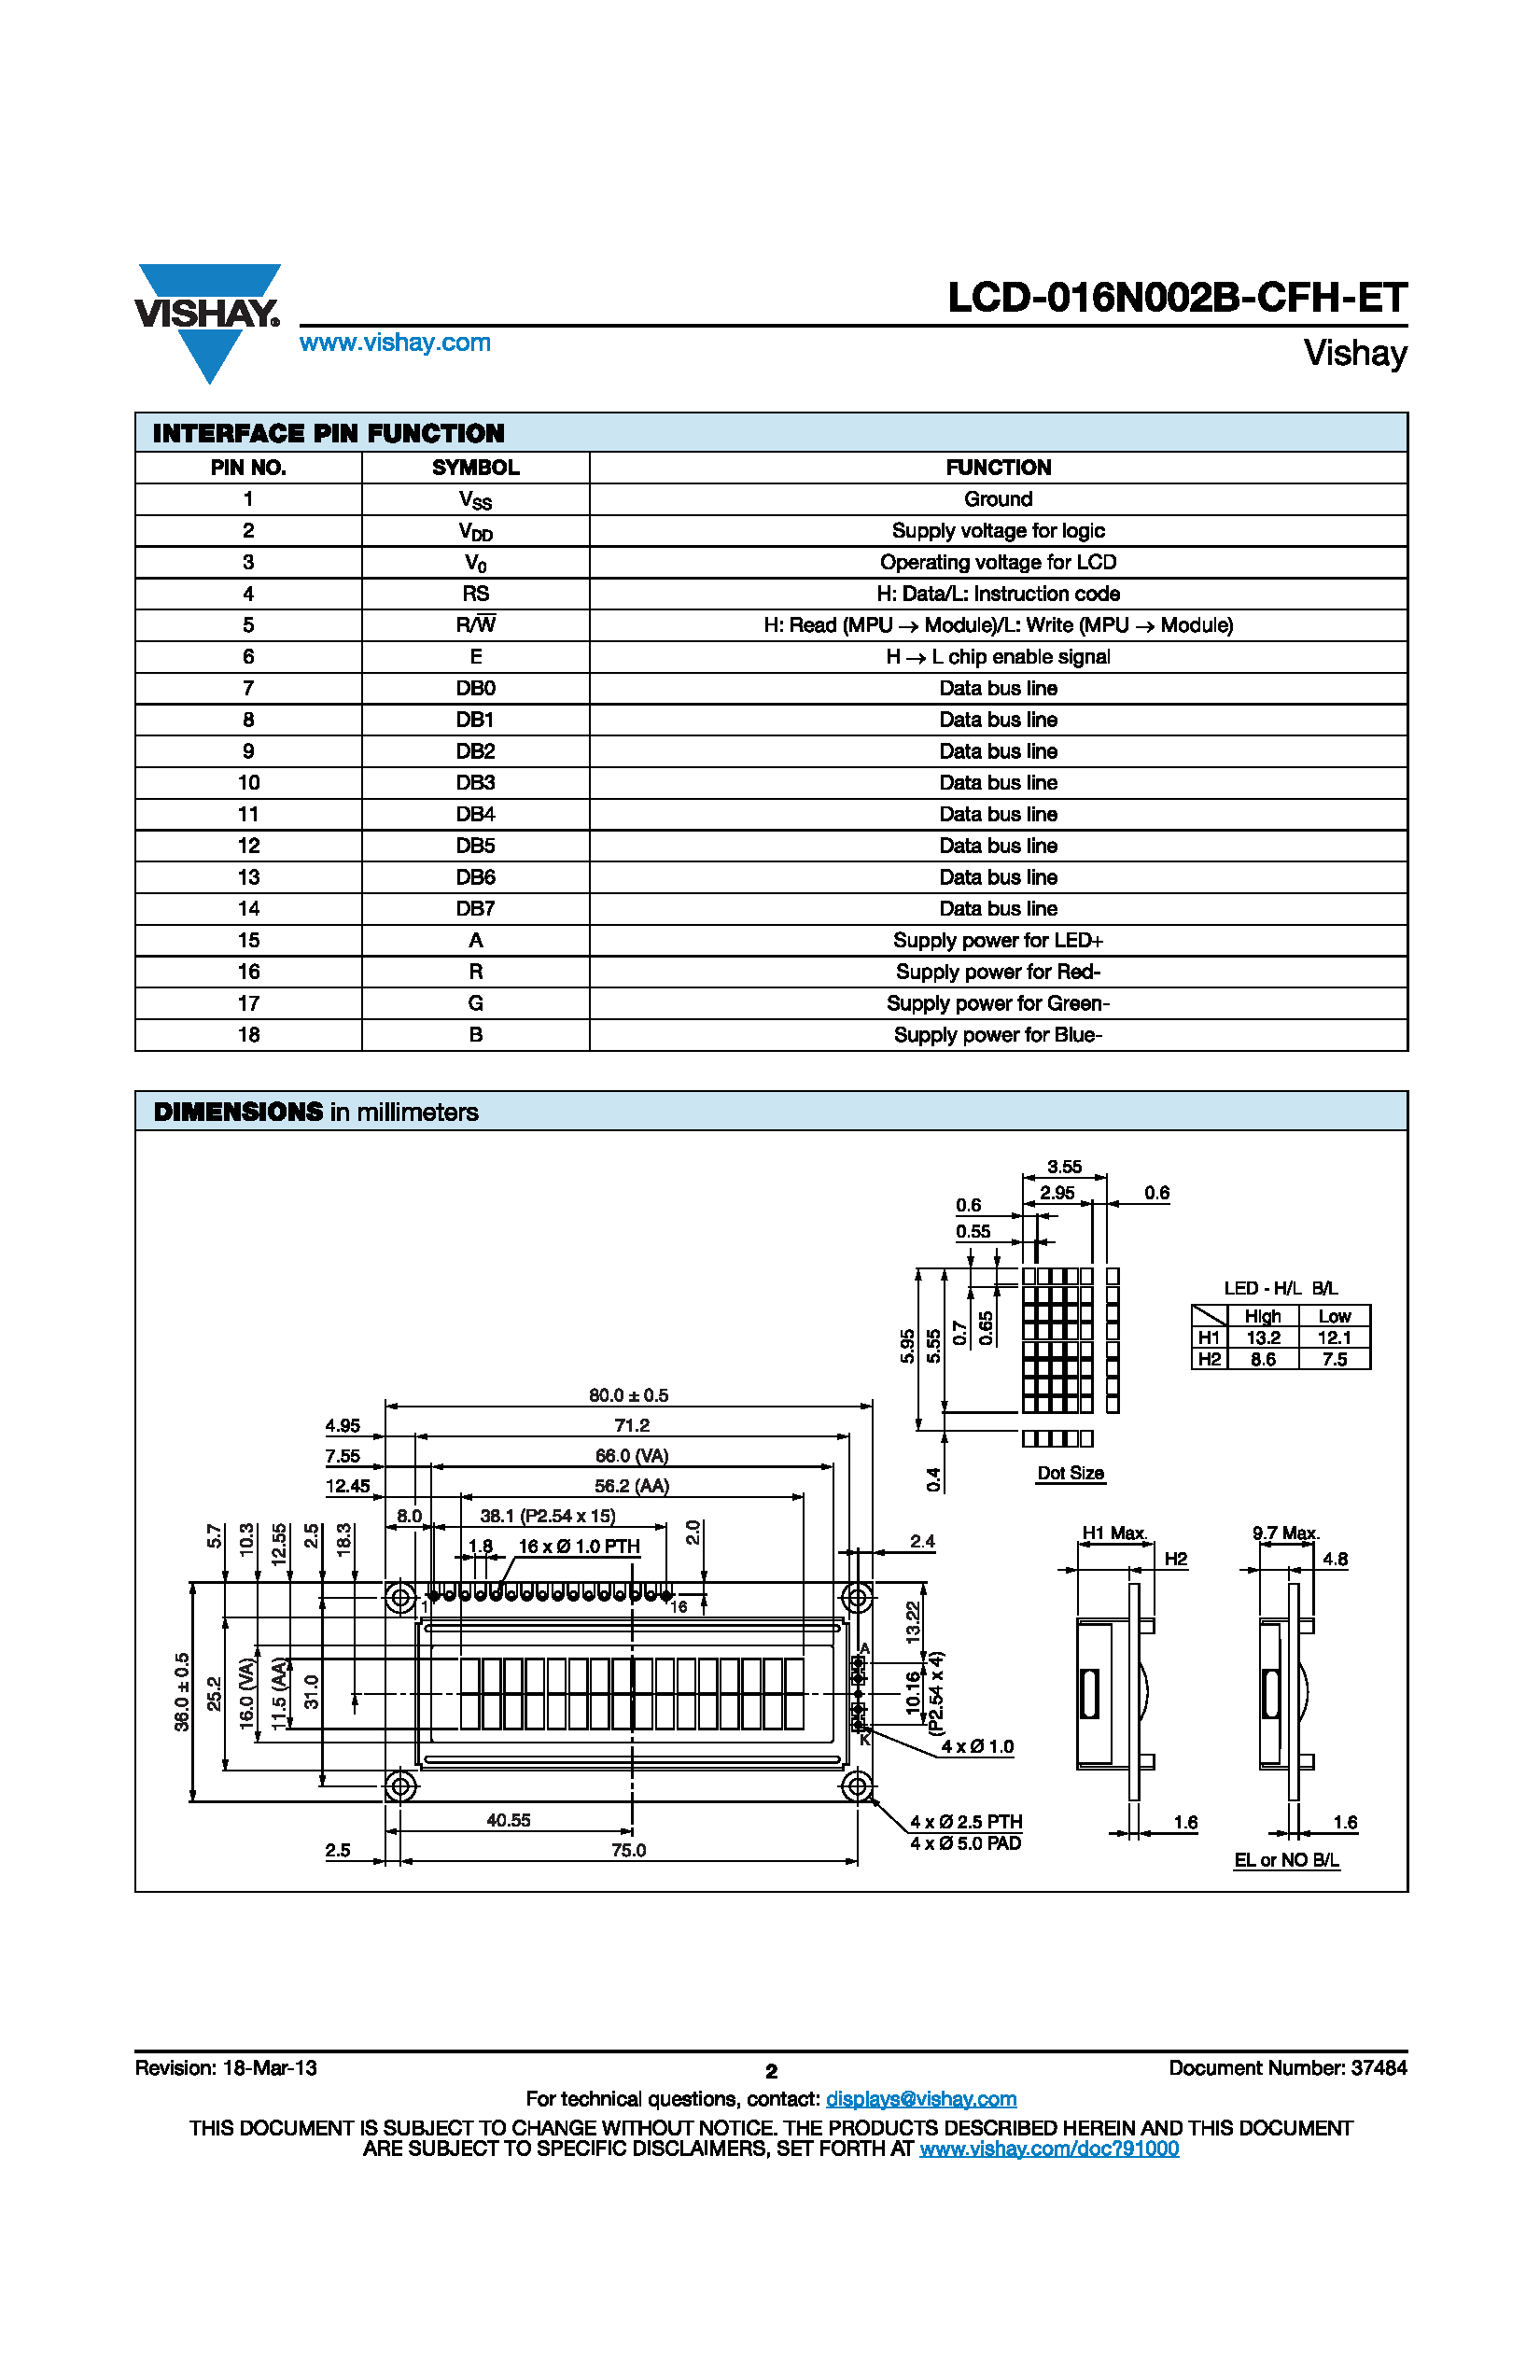
\includegraphics[trim = {30mm 250mm 90mm 20mm},clip,scale=0.5]{6/Img/lcd-16x2.pdf}
    %     \caption{Esquema LCD de 16x2}
    %     \label{fig:lcd-16x2}
    % \end{figure}
    % 
    % 
    \subsection{Prepara tu documento}
    
    Antes de que comiences a utilizar esta plantilla, es recomendable que prepare la información que contendrá en un archivo aparte. 
    Ten preparadas tus gráficas, así como también las tablas aparte, para que sea más fácil integrarlo. 
    Se recomienda fuertemente el uso de \textbf{formato Enhanced Metafile (.emf) para imágenes y gráficas} de resolución óptima. 
    Finalmente, completa y organiza el contenido antes de darle el formato de esta plantilla. 
    
    \subsection{Acrónimos y Abreviaciones}
    
    Los acrónimos y abreviaciones deberán ser definidos únicamente la primera vez que aparecen en el texto, esto para que el lector entienda lo que significan.
    
    \subsection{Ecuaciones}
    
    Las ecuaciones son una excepción a las especificaciones prescritas de esta plantilla. 
    Deberá determinar si su ecuación debe escribirse o no utilizando la fuente Adobe Devangari. 
    Para crear ecuaciones multinivel, puede ser necesario tratar la ecuación como un gráfico e insertarla en el texto después de aplicar el estilo de la platilla.
    Las ecuaciones serán enumeradas de manera consecutiva, y el número de ecuación, entre paréntesis, se colocan al ras de la derecha, utilizando una tabulación derecha. 
    
    \begin{equation}
        \label{eq1}
        x + y = z 
    \end{equation}
    
    Es importante asegurarse de que los símbolos de la ecuación sean definidos antes o inmediatamente después de la ecuación. Utilice “(1)”, en vez de “Eq. 1” al enumerar las ecuaciones, excepto al principio de una oración: “La ecuación (\ref{eq1}) es…”
    
    \section{Resultados y discusión}
    
    Antes de comenzar a preparar tu artículo, es importante que lea primero la guía del autor, la cual incluye los temas o apartados que son necesarios para tener tu trabajo completo.
    Una vez completada la edición del texto, el documento está listo para el uso de esta plantilla. En este archivo recién creado, resalte todo el contenido e importe el archivo de texto preparado. Ahora esta listo para estilizar su documento.
    En esta sección se deben presentar todo lo obtenido de la sección 2, incluidas deducciones o efectos del desarrollo. También se podrán incluir subsecciones numeradas de la siguiente forma:
    
    \subsection{Autores y Afiliaciones}
    
    Para distinguir las afiliaciones de los autores, utilice superíndices iniciando con el número 1, 2, etc., sucesivamente, esto dependerá de la cantidad de los departamentos a los que estén afiliados los autores. En caso de que todos los autores pertenezcan a una mismo departamento e institución, utilizar sólo el superíndice 1. 
    
    \subsection{Identificar los encabezados}
    
    Se les recuerda a los autores que los encabezados deben de estar conforme los solicita la guía del autor. De ahí se puede adaptar el trabajo para que sea más fácil de entender para el lector.
    Los encabezados organizan los temas sobre una base relacional y jerárquica. Por ejemplo, el título del documento es encabezado del texto principal porque todo el material posterior se relaciona y elabora sobre este tema. 
    
    \subsection{Tablas y Figuras}
    
    \begin{enumerate}
        \item Posición de las tablas y figuras: Coloque las figuras y las tablas en la parte superior e inferior de las columnas. Evite colocarlos en medio. Las figuras y las tablas grandes pueden abarcar ambas columnas. Los títulos de las figuras deben de estar debajo de las mismas; los títulos de las tablas deben aparecer encima de ellas. Insértese las figuras y los cuadros después de citarse en el texto. Utilice la abreviatura “Fig. 1”, incluso al principio de una oración. 
    \end{enumerate}
    
    \section{Conclusiones}
    
    Se describe aquí el alcance del trabajo, logros obtenidos y perspectivas para el futuro de este. Se sugiere colocar información cuantitativa obtenida.
    
    \section{Agradecimientos}
    
    Es importante darles su debido reconocimiento a los laboratorios, instituciones, organizaciones, entre otros que han sido participes para la culminación de este trabajo. También es importante mencionar, fondos, proyectos, becas, entre otros que se le han otorgado al o los autores para realizar el trabajo de investigación. Ejemplo: “Los autores agradecen al Concejo Nacional de Ciencia y Tecnología por los recursos otorgados…”
    
    \section*{Referencias}
    
    Para esta platilla, se solicita al autor enumerar las citas de manera consecutiva entre corchetes \cite{YLi2013}. 
    La puntuación de la oración que sigues sería \cite{Mesaelides2011}. 
    Refiérase simplemente al número de referencia, como en \cite{Morales2012}, no utilice “Ref. [3]” o “referencia [3]” excepto al principio de una oración: “La referencia [3] fue la primera…”
    Enumere las notas al pie por separado en superíndices. Coloque la nota de pie de en la parte inferior de la columna en la que se citó. No coloque notas al pie en la lista de referencias. Utilice letras para las notas al pie de la tabla.
    A menos de que haya tres autores o más; no utilice “et al.”. Los trabajos que no hayan sido publicados, incluso si han sido presentados para su publicación, deben ser citados como “inéditos”. Los trabajos que han sido aceptados para su publicación deben de citarse como “en prensa”. Poner en mayúscula sólo la primera palabra de un título, excepto los nombres propios y los símbolos de elemento. 
    Otros ejemplos \cite{LAAngeles2021}, \cite{LAAngelesConni}. 
    Véase el archivo adjunto \ref{anexo:pines}.
    
    % Ejemplo
    %  @Article{article,
    % 	author = "Author1 LastName1 and Author2 LastName2 and Author3 LastName3",
    % 	title = "Article Title",
    % 	volume = "30",
    % 	number = "30",
    % 	pages = "10127-10134",
    % 	year = "2013",
    % 	doi = "10.3389/fnins.2013.12345",
    % 	URL = "http://www.frontiersin.org/Journal/10.3389/fnins.2013.12345/abstract",
    % 	journal = "Frontiers in Neuroscience"
    % }
    
    % @book{book,
    %   author    = {Author Name}, 
    %   title     = {The title of the work},
    %   publisher = {The name of the publisher},
    %   address   = {The city},
    %   year      = 1993,
    % }
    
    % @incollection{chapter,
    %   author       = {Bauthor Surname}, 
    %   title        = {The title of the work},
    %   editor       = {Editor Name},
    %   booktitle    = {The title of the book},
    %   publisher    = {The name of the publisher},
    %   address      = {The city},
    %   year         = 2002,
    %   pages        = {201-213},
    % }
    
    % @InProceedings{conference,
    %   author = {Cauthor Name and Dauthor Surname and Fauthor LastName},
    %   title = {The title of the work},
    %   booktitle = {The title of the conference proceedings},
    %   year = 1996,
    %   publisher = {The name of the publisher},
    %   editor = {Editor Name1 and Editor Name2},
    %   pages = {41-50},
    % }
    
    % @book{cho,
    %   author       = {Gauthor Name1}, 
    %   title        = {The title of the work},
    %   publisher = {Country code and patent number},
    %   address      = {Patent Country},
    %   year = 2013
    % }
    
    % @book{patent,
    %   author    = {Hauthor Surname1}, 
    %   title     = {The title of the work},
    %   publisher = {Patent number},
    %   address   = {Patent country},
    %   year      = 2010,
    % }
    
    % % please use misc for datasets
    % @misc{dataset, 
    % 	author = "Author1 LastName1 and Author2 LastName2 and Author3 LastName3",
    % 	title = "Data Title",
    % 	year = "2011",
    % 	doi = "10.000/55555",
    % 	URL = "http://www.frontiersin.org/",
    % }
    
    \bibliographystyle{ieeetr}
    \bibliography{6/referencias}
    % 
    % 
    %%%%%%%%%%%%%%%%%%%%%%%%%%%%%%%%%%
    \appendix
    %%%%%%%%%%%%%%%%%%%%%%%%%%%%%%%%%%
    % 
    % 
    \centering{\section[\appendixautorefname{}]{APÉNDICE}}
    % \includepdf[pages=-]{6/Img/pines.pdf}
    \label{anexo:pines}
    %%%%%%%%%%%%%%%%%%%%%%%%%%%%%%%%%%%%%%%%
    \lhead{\begin{tikzpicture}[remember picture, overlay]
        \node [anchor=100,inner sep=0] (imagenIZQUIERDA) at (current page header area.north){
\includegraphics[width=18cm]{img/Encabezado.PNG}};
        \end{tikzpicture}}
        \rhead{Ángeles-Hurtado}
        \rfoot{\begin{tikzpicture}[remember picture, overlay]
        \node [anchor=140,inner sep=0] (imagenDERECHA) at (current page footer area.south){
\includegraphics[width=18cm]{img/Foot.PNG}};
        \end{tikzpicture}}
        %----------------------------------------------------------------------------------------
        \lfoot{ \thepage}
        % \renewcommand{\labelenumi}{\alph{enumi}.)} 
        %----------------------------------------------------------------------------------------
        %----------------------------------------------------------------------------------------
        %	TITLE SECTION
        %----------------------------------------------------------------------------------------
        
        \setlength{\droptitle}{-5\baselineskip} % Move the title up
        \title{\textbf{Estudio de tiempos y movimientos en el ensamble de un circuito electrónico utilizando diferentes métodos para su optimización }} % Article title
        
         \author{ 
         \textsc{Sáenz-Saavedra, Kenia Paola}\\ 
        %  Afiliación:
         \texttt{ Instituto Tecnológico de Querétaro } \\ 
         \texttt{Tecnológico Nacional de México} \\ 
         \texttt{Querétaro, México}\\ 
         \texttt{l22140911@queretaro.tecnm.mx} 
         \and 
         \textsc{Ángeles-Hurtado, Luis Alberto}\\ 
        %  Afiliación:
         \texttt{ Instituto Tecnológico de Querétaro } \\ 
         \texttt{ Tecnológico Nacional de México } \\ 
         \texttt{Querétaro, México}\\ 
         \texttt{alb3rt0.ah@gmail.com} 
        }
        
        
        %----------------------------------------------------------------------------------------
        
        % \begin{document}
        
        % Print the title
        \maketitle
        \thispagestyle{fancy}
        
        %----------------------------------------------------------------------------------------
        %	ARTICLE CONTENTS
        %----------------------------------------------------------------------------------------
        
        % \section*{Resumen}
        % \textit{Palabras clave:}
        % El resumen (ancho de página) deberá contener entre 100 y 200 palabras tipo Adobe Devangari 11 puntos.
        
        \begin{abstract}
        \noindent 
        El resumen (ancho de página) deberá contener entre 100 y 200 palabras tipo Adobe Devangari 11 puntos.
        
        \end{abstract}
        % 
        % 
        \textbf{\textit{Palabras clave}}: {First keyword should be the corresponding to the research area according with the authors guide. Maximum of 6 keywords.}
        % \keywords{First keyword should be the corresponding to the research area according with the authors guide. Maximum of 6 keywords.}
        \begin{itemize}
            \item Estándar, preciso, exacto, optimización, proceso.
        \end{itemize}
        
        \section{Introducción}
        
        %begin{itemize}
        
        El estudio de tiempos y movimientos es una herramienta la cual sirve para determinar los tiempos estándar de cada una de las operaciones que componen cualquier proceso, así como para analizar los movimientos que son realizados por parte de un operario para llevar a cabo dicha operación.
        
        A finales del siglo XIX, Frederick Taylor comenzó a estudiar los tiempos asociados con actividades laborales y desarrolló el concepto de tarea. Motivados por los estudios de tiempos de Taylor, alrededor del mismo periodo, la pareja de esposos Frank y Lillian Gilbreth condujeron estudios de movimientos (Krenn, 2011) que complementaron el trabajo de Taylor sobre estudios de tiempos. 
        \cite{andrade2019estudio}
        
        El ensamble que se analizará en este estudio de tiempos es un circuito  que es una colección de elementos eléctricos interconectados de alguna forma específica. Este circuito se estudiará a través de un Método de tiempos predeterminados. Consisten una base de datos de tiempos de movimientos básicos.Se asignan tiempos estándar a los elementos básicos del trabajo. Se asignan a los movimientos fundamentales y a grupos de movimientos que no se pueden evaluar con precisión mediante los procedimientos ordinarios de estudio de tiempos con cronómetro. También son el resultado de estudiar una muestra grande de operaciones diversificadas con un dispositivo de ritmo como una cámara de filmación o vídeo-grabación, capaz de medir elementos muy cortos.
        
        El estudio que se realiza en este proyecto integrador tuvo cómo objetivo principal llevar a la práctica los conocimientos adquiridos a lo largo de estos 4 semestres, involucrando las materias y talleres ya cursados en la carrera. De igual manera a través de este ensamble desarrollar nuevas habilidades adquiridas en la materia de Estudió del Trabajo II. Aplicando lo anterior mencionado, obtener buenos resultados a través del del estudio, buscando  una optimización en este proceso, que es buscar la mejor manera de realizar una actividad, lo más eficientemente posible, con la menor cantidad de recursos.
        
        El estudio de tiempos con cronómetro de forma tradicional, representa la técnica más utilizada como elemento de medición de las tareas, encontrándose más del 89\% de los trabajos desarrollados bajo ésta técnica.
        La aplicación del estudio de tiempos y movimientos sigue teniendo vigencia en la actualidad, como lo demuestran las 66 investigaciones realizadas entre los años 2010–2016, las cuales aplicaron las técnicas de medición del trabajo en sus formas tradicionales de muestreo del trabajo, estudio de tiempos con cronómetro y estándares de tiempo predeterminados.
        
        %endi{itemize}
         
        % Define estudio de tiempos y movimientos
        % define que es ensamble
        % define que es circuito electronico
        % define el metodo de tiempos predeterminados
        % define optimización
        % 
        % 
        \section{Justificación}
        
        %\begin{itemize}
        El entorno global ha llevado a las organizaciones a buscar la mejora de sus procesos por medio de la identificación y eliminación en forma gradual de las actividades que no generan valor a sus productos y procesos. Estas actividades representan costos operacionales que se traducen en despilfarros de tiempo, materiales, espacio y demás recursos organizacionales. Una de las técnicas más utilizadas para superar dichas deficiencias y elevar la productividad de los trabajadores es el estudio del trabajo.
            
        
        %\end{itemize}
        % 
        % 
        \section{Descripción del problema}
        \begin{itemize}
            \item Se debe describir la desviación o diferencia del ``es'' con respecto al ``debe ser''.
            \item Se debe hacer alusión a la incógnita científica*.
            \item Debe de tener Referencias científicas, URL, tesis, etc.
        \end{itemize}
        
        \textbf{*La incógnita científica es el elemento cuya solución incrementa el conocimiento científico.}
        % 
        % 
        \section{Fundamentación teórica}
        
        Es la parte medular y de mayor discusión, deberá ser la fundamentación de la hipótesis, por tanto se deberá señalar claramente la razón de la suposición y fundamentación de la misma. Únicamente referencias científicas.
        \begin{itemize}
            \item Se debe de retomar el tema que se planteo en la introducción, pero ahora profundizando para clarificar la incógnita científica y se pueda plantear la hipótesis.
            \item Se debe de retomar la descripción del problema, pero ahora a profundidad del (los) objeto(s) de estudio. 
            \item Se debe de profundizar en las metodologías que se ha usado para el estudio del tema.
            \item Referencias solo de artículos y libros científicos.
        \end{itemize}
        % 
        % 
        \section{Hipótesis}
        
        Es la suposición con fundamento científico relativa a la solución del problema, necesidad o de cómo se aprovecha la oportunidad con la incógnita científica y se fundamenta con: 1. Una suposición (en afirmativo o negativo) y ésta deberá vincularse con:
        2. La fundamentación científica que deberá ser precisa 3. Una entidad de comparación para probar la suposición y
        4. La variable con que se califica o cuantifica la comparación o se prueba la hipótesis.
        
        \begin{itemize}
            \item Se debe de identificar claramente la suposición científica
            \item Se debe de identificar claramente el fundamento científico
            \item Se debe identificar claramente la variable de respuesta
            \item Se debe identifican claramente las realidades o modelos contrastantes
            \item Se debe de establecer las variables asociadas, explicativas o que tienen relación funcional con la variable de respuesta
        \end{itemize}
        % 
        % 
        \section{Objetivo}
        
        Realizar un estudio de tiempos y movimientos de un ensamble eléctrico para a partir de este análisis eliminar los movimientos ineficientes, eliminar tiempos muertos y aumentar la productividad, de esta manera comprobando la hipótesis planteada.
        
        
        \subsection{Objetivos específicos }
        
        \begin{itemize}
            \item Diseña, mejora e integra sistemas productivos de bienes y servicios aplicando tecnologías para su optimización
            \item Diseña, implementa y mejora sistemas de trabajo para elevar la productividad.
        \end{itemize}
        
        
        % 
        \section{Cuerpo (Metodología, modelo matemático, etc.)}
        
        
        
        %\begin{itemize}
        
        En la elaboración de este proyecto, es necesario establecer que se cumplirán con los objetivos descritos anteriormente. Para el diseño y la mejora en sistemas productivos, de manera De manera sistemática, se analizarán los procesos existentes y se identificarán áreas de mejora utilizando herramientas de análisis, en este caso se realizará un estudio de tiempos y movimientos. Se llevarán a cabo las mejoras propuestas utilizando metodologías ágiles, esto apoyándonos de diferentes software y de un cronometro para la medición del tiempo en ciclos.
        
        
        Para el diseño, implementación y mejora de los sistemas se realizarán análisis detallados de los flujos de trabajo actuales, identificando cuellos de botella y oportunidades de mejora.Se pondrán en práctica nuevas metodologías de trabajo, como el trabajo en equipo colaborativo y la gestión ágil de proyectos.
        
        
        Se establecerán sistemas de retroalimentación para recopilar comentarios de los operarios que realizarán el ensamble para conocer sus incomodidades y retrasos en el proceso, así realizar los ajustes necesarios.Se aplicará el método de estudio de tiempos y movimientos para optimizar la eficiencia de las operaciones.
        
        Se elaborará un manual en dónde se describirá cada herramienta, equipo, maquina y todos los pasos que el operador debe de seguir para llegar al ensamble final. Se realizará un estudio de tiempos con ayuda del cronómetro y en base a esto se harán mejoras. A continuación se muestra el manual.
        
        %\end{itemize}
        
        
        
        
        %%%%%%%%%%%%%%%%%%%%%%%%%%%%%%%%%%
        \appendix
        %%%%%%%%%%%%%%%%%%%%%%%%%%%%%%%%%%
        % 
        % 
        % \section[\appendixname~\thesection]{Apéndice}
        \centering{\section[\appendixautorefname{manualEnsambleEléctrico.pdf }]{}}
        
        \includepdf[pages=-]{32/Img/manualEnsambleEléctrico.pdf}
        \label{anexo:manualEnsambleEléctrico.pdf}
        %%%%%%%%%%%%%%%%%%%%%%%%%%%%%%%%%%%%%%%%
        
        
        
        
        
        \subsection{Prepara tu documento}
        
        Antes de que comiences a utilizar esta plantilla, es recomendable que prepare la información que contendrá en un archivo aparte. 
        Ten preparadas tus gráficas, así como también las tablas aparte, para que sea más fácil integrarlo. 
        Se recomienda fuertemente el uso de \textbf{formato Enhanced Metafile (.emf) para imágenes y gráficas} de resolución óptima. 
        Finalmente, completa y organiza el contenido antes de darle el formato de esta plantilla. 
        
        \subsection{Acrónimos y Abreviaciones}
        
        Los acrónimos y abreviaciones deberán ser definidos únicamente la primera vez que aparecen en el texto, esto para que el lector entienda lo que significan.
        
        \subsection{Ecuaciones}
        
        Las ecuaciones son una excepción a las especificaciones prescritas de esta plantilla. 
        Deberá determinar si su ecuación debe escribirse o no utilizando la fuente Adobe Devangari. 
        Para crear ecuaciones multinivel, puede ser necesario tratar la ecuación como un gráfico e insertarla en el texto después de aplicar el estilo de la platilla.
        Las ecuaciones serán enumeradas de manera consecutiva, y el número de ecuación, entre paréntesis, se colocan al ras de la derecha, utilizando una tabulación derecha. 
        
        \begin{equation}
            \label{eq1}
            x + y = z 
        \end{equation}
        
        Es importante asegurarse de que los símbolos de la ecuación sean definidos antes o inmediatamente después de la ecuación. Utilice “(1)”, en vez de “Eq. 1” al enumerar las ecuaciones, excepto al principio de una oración: “La ecuación (\ref{eq1}) es…”
        
        \section{Resultados y discusión}
        
        Antes de comenzar a preparar tu artículo, es importante que lea primero la guía del autor, la cual incluye los temas o apartados que son necesarios para tener tu trabajo completo.
        Una vez completada la edición del texto, el documento está listo para el uso de esta plantilla. En este archivo recién creado, resalte todo el contenido e importe el archivo de texto preparado. Ahora esta listo para estilizar su documento.
        En esta sección se deben presentar todo lo obtenido de la sección 2, incluidas deducciones o efectos del desarrollo. También se podrán incluir subsecciones numeradas de la siguiente forma:
        
        \subsection{Autores y Afiliaciones}
        
        Para distinguir las afiliaciones de los autores, utilice superíndices iniciando con el número 1, 2, etc., sucesivamente, esto dependerá de la cantidad de los departamentos a los que estén afiliados los autores. En caso de que todos los autores pertenezcan a una mismo departamento e institución, utilizar sólo el superíndice 1. 
        
        \subsection{Identificar los encabezados}
        
        Se les recuerda a los autores que los encabezados deben de estar conforme los solicita la guía del autor. De ahí se puede adaptar el trabajo para que sea más fácil de entender para el lector.
        Los encabezados organizan los temas sobre una base relacional y jerárquica. Por ejemplo, el título del documento es encabezado del texto principal porque todo el material posterior se relaciona y elabora sobre este tema. 
        
        \subsection{Tablas y Figuras}
        
        \begin{enumerate}
            \item Posición de las tablas y figuras: Coloque las figuras y las tablas en la parte superior e inferior de las columnas. Evite colocarlos en medio. Las figuras y las tablas grandes pueden abarcar ambas columnas. Los títulos de las figuras deben de estar debajo de las mismas; los títulos de las tablas deben aparecer encima de ellas. Insértese las figuras y los cuadros después de citarse en el texto. Utilice la abreviatura “Fig. 1”, incluso al principio de una oración. 
        \end{enumerate}
        
        \section{Conclusiones}
        
        Se describe aquí el alcance del trabajo, logros obtenidos y perspectivas para el futuro de este. Se sugiere colocar información cuantitativa obtenida.
        
        \section{Agradecimientos}
        
        Es importante darles su debido reconocimiento a los laboratorios, instituciones, organizaciones, entre otros que han sido participes para la culminación de este trabajo. También es importante mencionar, fondos, proyectos, becas, entre otros que se le han otorgado al o los autores para realizar el trabajo de investigación. Ejemplo: “Los autores agradecen al Concejo Nacional de Ciencia y Tecnología por los recursos otorgados…”
        
        \section*{Referencias}
        
        Para esta platilla, se solicita al autor enumerar las citas de manera consecutiva entre corchetes \cite{YLi2013}. 
        La puntuación de la oración que sigues sería \cite{Mesaelides2011}. 
        Refiérase simplemente al número de referencia, como en \cite{Morales2012}, no utilice “Ref. [3]” o “referencia [3]” excepto al principio de una oración: “La referencia [3] fue la primera…”
        Enumere las notas al pie por separado en superíndices. Coloque la nota de pie de en la parte inferior de la columna en la que se citó. No coloque notas al pie en la lista de referencias. Utilice letras para las notas al pie de la tabla.
        A menos de que haya tres autores o más; no utilice “et al.”. Los trabajos que no hayan sido publicados, incluso si han sido presentados para su publicación, deben ser citados como “inéditos”. Los trabajos que han sido aceptados para su publicación deben de citarse como “en prensa”. Poner en mayúscula sólo la primera palabra de un título, excepto los nombres propios y los símbolos de elemento. 
        Otros ejemplos \cite{LAAngeles2021}, \cite{LAAngelesConni}. 
        Véase el archivo adjunto \ref{anexo:pines}.
        
        % Ejemplo
        %  @Article{article,
        % 	author = "Author1 LastName1 and Author2 LastName2 and Author3 LastName3",
        % 	title = "Article Title",
        % 	volume = "30",
        % 	number = "30",
        % 	pages = "10127-10134",
        % 	year = "2013",
        % 	doi = "10.3389/fnins.2013.12345",
        % 	URL = "http://www.frontiersin.org/Journal/10.3389/fnins.2013.12345/abstract",
        % 	journal = "Frontiers in Neuroscience"
        % }
        
        % @book{book,
        %   author    = {Author Name}, 
        %   title     = {The title of the work},
        %   publisher = {The name of the publisher},
        %   address   = {The city},
        %   year      = 1993,
        % }
        
        % @incollection{chapter,
        %   author       = {Bauthor Surname}, 
        %   title        = {The title of the work},
        %   editor       = {Editor Name},
        %   booktitle    = {The title of the book},
        %   publisher    = {The name of the publisher},
        %   address      = {The city},
        %   year         = 2002,
        %   pages        = {201-213},
        % }
        
        % @InProceedings{conference,
        %   author = {Cauthor Name and Dauthor Surname and Fauthor LastName},
        %   title = {The title of the work},
        %   booktitle = {The title of the conference proceedings},
        %   year = 1996,
        %   publisher = {The name of the publisher},
        %   editor = {Editor Name1 and Editor Name2},
        %   pages = {41-50},
        % }
        
        % @book{cho,
        %   author       = {Gauthor Name1}, 
        %   title        = {The title of the work},
        %   publisher = {Country code and patent number},
        %   address      = {Patent Country},
        %   year = 2013
        % }
        
        % @book{patent,
        %   author    = {Hauthor Surname1}, 
        %   title     = {The title of the work},
        %   publisher = {Patent number},
        %   address   = {Patent country},
        %   year      = 2010,
        % }
        
        % % please use misc for datasets
        % @misc{dataset, 
        % 	author = "Author1 LastName1 and Author2 LastName2 and Author3 LastName3",
        % 	title = "Data Title",
        % 	year = "2011",
        % 	doi = "10.000/55555",
        % 	URL = "http://www.frontiersin.org/",
        % }
        
        \bibliographystyle{ieeetr}
        \bibliography{6/referencias}
        % 
        % 
        %%%%%%%%%%%%%%%%%%%%%%%%%%%%%%%%%%
        \appendix
        %%%%%%%%%%%%%%%%%%%%%%%%%%%%%%%%%%
        % 
        % 
        \centering{\section[\appendixautorefname{}]{APÉNDICE}}
        % \includepdf[pages=-]{6/Img/pines.pdf}
        \label{anexo:pines}
        %%%%%%%%%%%%%%%%%%%%%%%%%%%%%%%%%%%%%%%%